\begin{figure}[h]
	\centering
	\setlength{\resLen}{1.in}
	\setlength{\raiseLen}{0.4in}
	\addtolength{\tabcolsep}{-4pt}
	\begin{tabular}{cccc}
		  & SVBRDF maps & Optimization & Novel
		\\
		\raisebox{\raiseLen}{\rotatebox[origin=c]{90}{GT}} &
		\includegraphics[height=\resLen]{svbrdf/validation/optim/fake_038/ref/tex.jpg} &
		
\includegraphics[height=\resLen]{svbrdf/validation/optim/fake_038/ref/00.jpg} &
		\includegraphics[height=\resLen]{svbrdf/validation/optim/fake_038/ref/08.jpg}
		\\
		\raisebox{\raiseLen}{\rotatebox[origin=c]{0}{(1)}} &
		\includegraphics[height=\resLen]{svbrdf/validation/optim/fake_038/1000_1000/tex.jpg} &
		
\includegraphics[height=\resLen]{svbrdf/validation/optim/fake_038/1000_1000/00.jpg} &
		\includegraphics[height=\resLen]{svbrdf/validation/optim/fake_038/1000_1000/08.jpg}
		\\
		\raisebox{\raiseLen}{\rotatebox[origin=c]{0}{(2)}} &
		\includegraphics[height=\resLen]{svbrdf/validation/optim/fake_038/0_0/tex.jpg} &
		
\includegraphics[height=\resLen]{svbrdf/validation/optim/fake_038/0_0/00.jpg} &
		\includegraphics[height=\resLen]{svbrdf/validation/optim/fake_038/0_0/08.jpg}
		\\
		\raisebox{\raiseLen}{\rotatebox[origin=c]{0}{(3)}} &
		\includegraphics[height=\resLen]{svbrdf/validation/optim/fake_038/10_10/tex.jpg} &
		
\includegraphics[height=\resLen]{svbrdf/validation/optim/fake_038/10_10/00.jpg} &
		\includegraphics[height=\resLen]{svbrdf/validation/optim/fake_038/10_10/08.jpg}
	\end{tabular}
	\caption[Optimization strategy]{\label{fig:svbrdf:strategy}
		\textbf{Optimization strategy.} We evaluated three optimization strategies: (1) optimize $\bw^+$ first, then $\noise$; (2) jointly optimize $\bw^+$ and $\noise$; (3) alternate between $\bw^+$ and $\noise$ every 10 iterations. Strategy (1) causes artifacts during the optimization, and (2) brings more noise into the maps. Particularly, for textures with small features, (1) and (2) may drive the optimization to bad local minima while the per-pixel loss could still be very low. Strategy (3) appears to be a good compromise, giving us better results in most cases. Note: ``Opt.'' means an  optimized input view or its re-rendering, i.e. not a novel view.
	}
\end{figure}
